\section{KNTT - Lớp 11 - Ôn tập giữa học kì 1 - Đề 5}

\caulc

\Opensolutionfile{ans}[ans-ABCD]

%======== Câu 1
\begin{ex}%[1D1H1-3]%[KNTT - Lớp 11 - Ôn tập giữa học kì 1 - Đề 5]%[Quan Ón]
	\immini{
		Cho tam giác đều $ABC$. Khẳng định nào sau đây \textbf{sai}?
		\choice
		{$\textrm{sđ}(BA,BC) = -60^{\circ}$}
		{$\textrm{sđ}(AB,AC) = -300^{\circ} + k360^{\circ}$ $(k \in \mathbb{Z})$}
		{\True $\textrm{sđ}(AB,AC) = 60^{\circ} + k180^{\circ}$ $(k \in \mathbb{Z})$}
		{$\textrm{sđ}(CB,CA) = 300^{\circ} + k360^{\circ}$ $(k \in \mathbb{Z})$}
	}{
		\begin{tikzpicture}[>=stealth,line join=round,line cap=round,font=\footnotesize,scale=1]
			%\clip (-2.4,-2.3) rectangle (2.4,4.6);
			\path 
			(0,0) coordinate (B)
			($(B) + (0:2.5)$) coordinate (C)
			($(B) + (60:2.5)$) coordinate (A)
			;
			\draw (B)--(A)--(C)--(B);
			\foreach \x/\g in {A/90,B/-135,C/-45}\fill[black] (\x) circle (1pt)+(\g:3mm) node{$ \x $};
		\end{tikzpicture}
	}
	\loigiai{
		Các góc lượng giác tia đầu $AB$, tia cuối $AC$ có số đo là $\textrm{sđ}(AB,AC) = 60^{\circ} + k360^{\circ}$ $(k \in \mathbb{Z})$.
	}
\end{ex}

%======== Câu 2
\begin{ex}%[1D1N3-2]%[KNTT - Lớp 11 - Ôn tập giữa học kì 1 - Đề 5]%[Quan Ón]
	Đẳng thức nào sau đây đúng?
	\choice
	{$\cos\left(\alpha + \dfrac{\pi}{3}\right) = \dfrac{1}{2}\cos\alpha + \dfrac{\sqrt{3}}{2}\sin\alpha$}
	{$\cos\left(\alpha + \dfrac{\pi}{3}\right) = \dfrac{1}{2}\sin \alpha - \dfrac{\sqrt{3}}{2}\cos\alpha$}
	{$\cos\left(\alpha + \dfrac{\pi}{3}\right) = \dfrac{\sqrt{3}}{2}\cos \alpha + \dfrac{1}{2}\sin\alpha$}
	{\True $\cos\left(\alpha + \dfrac{\pi}{3}\right) = \dfrac{1}{2}\cos\alpha - \dfrac{\sqrt{3}}{2}\sin\alpha$}
	\loigiai{
		Áp dụng công thức cộng, ta có
		$$\cos\left(\alpha + \dfrac{\pi}{3}\right) = \cos\alpha\cdot \cos\dfrac{\pi}{3} - \sin\alpha\cdot \sin\dfrac{\pi}{3} = \dfrac{1}{2}\cos\alpha - \dfrac{\sqrt{3}}{2}\sin\alpha.$$
	}
\end{ex}

%======== Câu 3
\begin{ex}%[1D1H2-2]%[KNTT - Lớp 11 - Ôn tập giữa học kì 1 - Đề 5]%[Quan Ón]
	Cho $\sin\alpha = \dfrac{3}{5}$, khi đó giá trị $\cos 2\alpha$ bằng
	\choice
	{$\dfrac{\sqrt{7}}{5}$}
	{$-\dfrac{7}{25}$}
	{$\dfrac{16}{25}$}
	{\True $\dfrac{7}{25}$}
	\loigiai{
		Ta có $\cos 2\alpha = 1 - 2\sin^2\alpha = 1 - 2\cdot\left(\dfrac{3}{5}\right)^2 = \dfrac{7}{25}$.
	}
\end{ex}	
	
%======== Câu 4
\begin{ex}%[1D1H4-2]%[KNTT - Lớp 11 - Ôn tập giữa học kì 1 - Đề 5]%[Quan Ón]
	Tập xác định của hàm số $y = \tan\left(2x+\dfrac{\pi}{3}\right)$ là
	\choice
	{$\mathscr{D} = \mathbb{R}\setminus\left\lbrace \dfrac{\pi}{12} + k\pi, k \in \mathbb{Z}\right\rbrace$}
	{\True $\mathscr{D} = \mathbb{R}\setminus\left\lbrace \dfrac{\pi}{12} + k\dfrac{\pi}{2}, k \in \mathbb{Z}\right\rbrace$}
	{$\mathscr{D} = \mathbb{R}\setminus\left\lbrace \dfrac{\pi}{6} + k\pi, k \in \mathbb{Z}\right\rbrace$}
	{$\mathscr{D} = \mathbb{R}\setminus\left\lbrace \dfrac{\pi}{12} + k2\pi, k \in \mathbb{Z}\right\rbrace$}
		\loigiai{
			Hàm số xác định khi
			$$
			\cos \left(2x + \dfrac{\pi}{3}\right) \neq 0 \Leftrightarrow 2x + \dfrac{\pi}{3} \neq \dfrac{\pi}{2} + k \pi \Leftrightarrow 2x \neq \dfrac{\pi}{6} + k\pi \Leftrightarrow x \neq \dfrac{\pi}{12} + k\dfrac{\pi}{2}.
			$$
			Vậy tập xác định $\mathscr{D} = \mathbb{R}\setminus\left\lbrace \dfrac{\pi}{12} + k \dfrac{\pi}{2}, k \in \mathbb{Z}\right\rbrace$.
		}
\end{ex}		
		
%======== Câu 5
\begin{ex}%[1D1N4-3]%[KNTT - Lớp 11 - Ôn tập giữa học kì 1 - Đề 5]%[Quan Ón]
	Trên khoảng $(-\pi; \pi)$ đồ thị hàm số $y = \sin x$ được cho như hình vẽ
	\begin{center}
		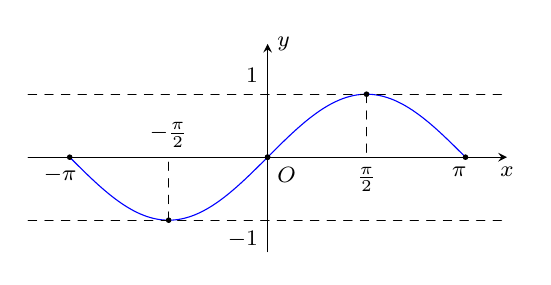
\begin{tikzpicture}[scale=0.8,>=stealth, font=\footnotesize, line join=round, line cap=round]
			\def\xmin{-3.8} \def\xmax{3.8} \def\ymin{-1.5} \def\ymax{1.8}
			\draw[->] (\xmin,0)--(\xmax,0) node [below]{$x$};
			\draw[->] (0,\ymin)--(0,\ymax) node [right]{$y$};
			\node at (0,0) [below right]{$O$};
			\draw[smooth,samples=400,domain=-3.14:3.14,color=blue] plot(\x,{sin(\x r)});
			\draw[dashed] (\xmin,1)--(\xmax,1) (\xmin,-1)--(\xmax,-1);
			\foreach \x in {-pi,-0.5*pi,0}
			{\draw[fill=black] (\x,sin \x*180/pi) circle (1pt);
				\draw[dashed] (\x,sin \x*180/pi)--(\x,0);
				\draw[fill=black] (-\x,sin -\x*180/pi) circle (1pt);
				\draw[dashed] (-\x,sin -\x*180/pi)--(-\x,0);}
			\node at (0,1.3) [left]{$1$};
			\node at (0,-1.3) [left]{$-1$};
			\node at (-pi-0.15,0) [below]{$-\pi$};
			\node at (-0.5*pi,0) [above]{$-\frac{\pi}{2}$};
			\node at (0.5*pi,0) [below]{$\frac{\pi}{2}$};
			\node at (pi-0.1,0) [below]{$\pi$};
		\end{tikzpicture}
	\end{center}
	Hỏi hàm số $y = \sin x$ nghịch biến trên khoảng nào sau đây?
	\choice
	{$(-\pi; 0)$}
	{$\left(-\dfrac{\pi}{2}; \dfrac{\pi}{2}\right)$}
	{$(0; \pi)$}
	{\True $\left(\dfrac{\pi}{2}; \pi\right)$}
	\loigiai{
		Từ hình vẽ, ta thấy đồ thị hàm số $y = \sin x$ \lq\lq đi xuống\rq\rq\, trên khoảng $\left(\dfrac{\pi}{2}; \pi\right)$, do đó hàm số nghịch biến trong khoảng $\left(\dfrac{\pi}{2}; \pi\right)$.
	}
\end{ex}			
			
%======== Câu 6
\begin{ex}%[1D1N5-5]%[KNTT - Lớp 11 - Ôn tập giữa học kì 1 - Đề 5]%[Quan Ón]
	Phương trình $\sin x = \dfrac{1}{2}$ có tập nghiệm là
	\choice
	{\True $S = \left\lbrace \dfrac{\pi}{6} + k2\pi; \dfrac{5\pi}{6} + k2\pi, k \in \mathbb{Z}\right\rbrace$}
	{$S = \left\lbrace \dfrac{\pi}{3} + k2\pi; -\dfrac{2\pi}{3} + k2\pi, k \in \mathbb{Z}\right\rbrace$}
	{$S = \left\lbrace \dfrac{\pi}{6} + k2\pi; -\dfrac{\pi}{6} + k2\pi, k \in \mathbb{Z}\right\rbrace$}
	{$S = \left\lbrace \dfrac{1}{6} + k2\pi, k \in \mathbb{Z}\right\rbrace$}
	\loigiai{
		Ta có $\sin x = \dfrac{1}{2} \Leftrightarrow \sin x = \sin\dfrac{\pi}{6} \Leftrightarrow \hoac{&x = \dfrac{\pi}{6} + k2\pi\\&x=\dfrac{5\pi}{6} + k2\pi} \quad (k \in \mathbb{Z})$.
	}
\end{ex}			
			
%======== Câu 7
\begin{ex}%[1D2N1-3]%[KNTT - Lớp 11 - Ôn tập giữa học kì 1 - Đề 5]%[Quan Ón]
	Cho dãy số $(u_n)$ với $u_n = \dfrac{17n - 6}{4n + 9}$, $\forall n \in \mathbb{N}^{*}$. Hỏi từ số hạng thứ $14$ của dãy số $(u_n)$ là bao nhiêu?
	\choice
	{$\dfrac{244}{47}$}
	{$\dfrac{227}{43}$}
	{$\dfrac{215}{61}$}
	{\True $\dfrac{232}{65}$}
	\loigiai{
		Ta có $u_{14} = \dfrac{17\cdot 14 - 6}{4\cdot 14 + 9} = \dfrac{232}{65}$.
	}
\end{ex}				
				
%======== Câu 8
\begin{ex}%[1D2N2-4]%[KNTT - Lớp 11 - Ôn tập giữa học kì 1 - Đề 5]%[Quan Ón]
	Cho cấp số cộng $(u_n)$ có $u_1 = 14$ và công sai $d = 2$. Tìm số hạng $u_4$.
	\choice
	{$u_4 = 22$}
	{\True $u_4 = 20$}
	{$u_4 = 8$}
	{$u_4 = 6$}
	\loigiai{
		Ta có $u_4 = u_1 + 3d = 14 + 3\cdot 2 = 20$.
	}
\end{ex}					
					
%======== Câu 9
\begin{ex}%[1D2N3-4]%[KNTT - Lớp 11 - Ôn tập giữa học kì 1 - Đề 5]%[Quan Ón]
	Cho cấp số nhân $(u_n)$ có $u_1 = -2$ và công bội $q = 3$. Số hạng $u_4$ là
	\choice
	{$u_4 = -6$}
	{\True $u_4 = -54$}
	{$u_4 = 1$}
	{$u_4 = -18$}
	\loigiai{
		Số hạng $u_4$ là $u_4 = u_1 \cdot q^3 = -2\cdot 3^3 = -54$.
	}
\end{ex}					
					
%======== Câu 10
\begin{ex}%[1H4N1-3]%[KNTT - Lớp 11 - Ôn tập giữa học kì 1 - Đề 5]%[Quan Ón]
	Cho hình chóp $S.ABCD$, biết $AC$ cắt $BD$ tại $O$, $AB$ cắt $CD$ tại $M$. Tìm giao tuyến của hai mặt phẳng $(SAB)$ và $(SCD)$.
	\choice
	{$SO$}
	{\True $SM$}
	{$SA$}
	{$SC$}
	\loigiai{
		\immini{
			Ta có $\heva{&M = AB\cap CD\\&AB \subset(SAB)\\&CD \subset (SCD)} \Rightarrow M \in (SAB) \cap (SCD)$.\\
			Lại có $S\in (SAB) \cap (SCD)$; $S\neq M$.\\
			Do đó $(SAB) \cap (SCD) = SM$.
		}{
			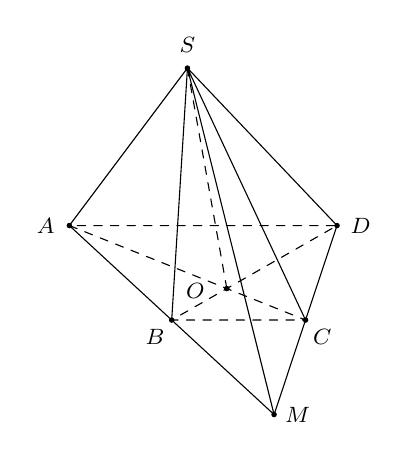
\begin{tikzpicture}[>=stealth,line join=round,line cap=round,font=\footnotesize,scale=1]
				\path 
				(0,0) coordinate (A)
				(1.3,-1.2) coordinate (B)
				(3,-1.2) coordinate (C)
				(3.4,0) coordinate (D)
				(1.5,2) coordinate (S)
				(intersection of A--C and D--B) coordinate (O)
				(intersection of A--B and D--C) coordinate (M)
				;
				\draw (B)--(A)--(S)--(B) (C)--(D)--(S)--(C) (B)--(M)--(C) (S)--(M);
				\draw[dashed] (A)--(C)--(B)--(D)--(A) (S)--(O);
				\foreach \x/\g in {A/180,B/-135,C/-45,D/0,S/90,M/0}\fill[black] (\x) circle (1pt)+(\g:3mm) node{$ \x $};
				\fill[black] (O) circle (1pt) + (185:4mm) node{$O$};
			\end{tikzpicture}
		}
	}
\end{ex}

%======== Câu 11
\begin{ex}%[1H4H1-4]%[KNTT - Lớp 11 - Ôn tập giữa học kì 1 - Đề 5]%[Quan Ón]
	Cho tứ giác $ABCD$ có $AC$ và $BD$ giao nhau tại $O$ và một điểm $S$ không thuộc mặt phẳng $(ABCD)$. Trên đoạn $SC$ lấy một điểm $M$ không trùng với $S$ và $C$. Giao điểm của đường thẳng $SD$ với mặt phẳng $(ABM)$ là
	\choice
	{giao điểm của $SD$ và $BM$}
	{giao điểm của $SD$ và $AM$}
	{\True giao điểm của $SD$ và $BK$}
	{giao điểm của $SD$ và $MK$}
	\loigiai{
		\immini{
			Chọn mặt phẳng phụ $(SBD)$ chứa $SD$.\\
			Tìm giao tuyến của hai mặt phẳng $(SBD)$ và $(ABM)$.\\
			Ta có $B$ là điểm chung thứ nhất của $(SBD)$ và $(ABM)$.\\
			Trong mặt phẳng $(SAC)$, gọi $K = AM\cap SO$. \\
			Ta có $\heva{&K\in AM, AM\subset(ABM)\\&K\in SO, SO\subset(SBD).}$\\
			Suy ra $K$ là điểm chung thứ hai của $(SBD)$ và $(ABM)$.\\
			Do đó $(SBD) \cap(ABM) = BK$.\\
			Trong mặt phẳng $(SBD)$, gọi $N = SD\cap BK$.\\
			Ta có $\heva{&N\in SD\\&N\in BK, BK\subset(ABM).}$\\
			Vậy $SD\cap (ABM) = N$.
		}{
			\begin{tikzpicture}[>=stealth,line join=round,line cap=round,font=\footnotesize,scale=1]
				\path 
				(0,0) coordinate (A)
				(0.6,-1) coordinate (B)
				(3,-1.6) coordinate (C)
				(4.2,0) coordinate (D)
				(1.5,2.6) coordinate (S)
				($(S)!0.4!(C)$) coordinate (M)
				(intersection of A--C and D--B) coordinate (O)
				(intersection of A--M and S--O) coordinate (K)
				(intersection of B--K and S--D) coordinate (N)
				;
				\draw (B)--(A)--(S)--(B) (C)--(D)--(S)--(C)--(B) (B)--(M);
				\draw[dashed] (C)--(A)--(D)--(B)--(N) (S)--(O) (A)--(M);
				\foreach \x/\g in {A/180,B/-90,C/-90,D/0,S/90,M/0,N/45,K/135}\fill[black] (\x) circle (1pt)+(\g:3mm) node{$ \x $};
				\fill[black] (O) circle (1pt)+(-95:2.5mm) node{$O$};
			\end{tikzpicture}
		}
	}
\end{ex}

%======== Câu 12
\begin{ex}%[1H4H2-2]%[KNTT - Lớp 11 - Ôn tập giữa học kì 1 - Đề 5]%[Quan Ón]
	Cho tứ diện $ABCD$. Gọi $I$, $J$ lần lượt là trọng tâm các tam giác $ABC$ và $ABD$. Khi đó $IJ$ song song với đường thẳng nào sau đây?
	\choice
	{$AB$}
	{\True $CD$}
	{$AC$}
	{$BD$}
	\loigiai{
		\immini{
			Gọi $M$, $N$ lần lượt là trung điểm của $BC$, $BD$\\
			$\Rightarrow MN$ là đường trung bình của tam giác $BCD$\\
			$\Rightarrow MN\parallel CD$. $\hspace*{1.2cm} (1)$\\
			$I$, $J$ lần lượt là trọng tâm các tam giác $ABC$ và $ABD$\\
			$\Rightarrow \dfrac{AI}{AM} = \dfrac{AJ}{AN} = \dfrac{2}{3} \Rightarrow IJ\parallel MN$. $\hspace*{1.2 cm} (2)$\\
			Từ $(1)$ và $(2)$ suy ra $IJ\parallel CD$.
		}{
			\begin{tikzpicture}[>=stealth,line join=round,line cap=round,font=\footnotesize,scale=1]
				\path 
				(1.2,2.4) coordinate (A)
				(0,0) coordinate (B)
				(3.8,0) coordinate (C)
				(1.6,-1.2) coordinate (D)
				($(B)!0.5!(C)$) coordinate (N)
				($(B)!0.5!(D)$) coordinate (M)
				($(A)!2/3!(M)$) coordinate (I)
				($(A)!2/3!(N)$) coordinate (J)
				;
				\draw (D)--(B)--(A)--(D)--(C)--(A)--(M);
				\draw[dashed] (C)--(B) (M)--(N)--(A) (I)--(J);
				\foreach \x/\g in {A/90,B/180,C/0,D/-90,M/-135,N/45,I/180,J/30}\fill[black] (\x) circle (1pt)+(\g:3mm) node{$ \x $};
			\end{tikzpicture}
		}
	}
\end{ex}						

\Closesolutionfile{ans}

\indapan{6}{ans-ABCD}

\cauds

\Opensolutionfile{ans}[ans-DS]

%======== Câu 1
\begin{ex}%[1D1H4-6]%[KNTT - Lớp 11 - Ôn tập giữa học kì 1 - Đề 5]%[Quan Ón]
	Cho hàm số $f(x) = \cos 2x + 2\sin x$. Các khẳng định sau đúng hay sai?
	\choiceTF
	{\True Hàm số $f(x)$ có tập xác định là $\mathbb{R}$}
	{Hàm số $f(x)$ là hàm số lẻ}
	{\True Chu kì tuần hoàn của hàm số $f(x)$ là $2\pi$}
	{Hàm số $f(x)$ có giá trị lớn nhất là $1$ và giá trị nhỏ nhất là $-3$}
	\loigiai{
		\begin{itemchoice}
			\itemch \textbf{Đúng}. Vì Hàm số $\cos 2x$ và $2\sin x$ đều có tập xác định là $\mathbb{R}$ nên hàm số $f(x)$ có tập xác định là $\mathbb{R}$.
			\itemch \textbf{Sai}. Ta có $\mathscr{D} = \mathbb{R} \Rightarrow \forall x \in \mathscr{D} \Rightarrow -x \in \mathscr{D}$.
			$$ f(-x) = \cos(-2x) + 2\sin(-x) = \cos 2x - 2\sin x. $$
			Nên $\heva{&f(-x) \neq f(x)\\&f(-x) \neq -f(x).}$\\
			Do đó hàm số $f(x)$ không chẵn, không lẻ.
			\itemch \textbf{Đúng}. Vì hàm số $\cos 2x$ tuần hoàn với chu kì $\pi$. Hàm số $\sin x$ tuần hoàn với chu kì $2\pi$ nên hàm số $f(x)$ tuần hoàn với chu kì $2\pi$.
			\itemch \textbf{Sai}. Ta có $f(x) = -2\sin^2x + 2\sin x + 1$.\\
			Đặt $t = \sin x$, điều kiện $-1 \leq t \leq 1$, ta được $f(t) = -2t^2 + 2t + 1$.\\
			Bảng biến thiên $f(t)$
			\begin{center}
				
\begin{tikzpicture}[scale=1, font=\footnotesize, line join=round, line cap=round, >=stealth]
					\tkzTabInit[nocadre=false,lgt=1.2,espcl=1.6,deltacl=0.8]
					{$t$ /1,$f(t)$ /1.6}
					{$-1$,$\dfrac{1}{2}$,$1$}
					\tkzTabVar{-/$-3$,+/$\dfrac{3}{2}$,-/$1$}
				\end{tikzpicture}
			\end{center}
			Giá trị lớn nhất của hàm số là $\dfrac{3}{2}$, giá trị nhỏ nhất của hàm số là $-3$.
		\end{itemchoice}
	}
\end{ex}

%======== Câu 2
\begin{ex}%[1D2H2-6]%[KNTT - Lớp 11 - Ôn tập giữa học kì 1 - Đề 5]%[Quan Ón]
	Cho cấp số cộng $(a_n)$ có ba số hạng đầu tiên của dãy là $1$, $3$, $5$ và cấp số nhân $(b_n)$ có ba số hạng đầu tiên của dãy là $3$, $6$, $12$.
	\choiceTF
	{\True Dãy cấp số cộng $(a_n)$ có công sai $d = 2$}
	{\True Số hạng thứ $10$ của dãy cấp số cộng $(a_n)$ là $19$}
	{Số $486$ thuộc dãy cấp số nhân $(b_n)$}
	{\True Tổng của $10$ số hạng đầu tiên của dãy cấp số nhân $(b_n)$ bằng $3069$}
	\loigiai{
		\begin{itemchoice}
			\itemch \textbf{Đúng}. Công sai của cấp số cộng $(a_n)$ là $d = a_2 - a_1 = 3 - 1 = 2$.
			\itemch \textbf{Đúng}. Số hạng thứ $10$ của dãy cấp số cộng $(a_n)$ là
			$$ a_{10} = a_1 + (10 - a)\cdot d = 1 + (10 - 1)\cdot 2 = 19. $$
			\itemch \textbf{Sai}. Giả sử số $486$ là số thứ $n$ của dãy cấp số nhân $(b_n)$. Khi đó
			$$ 486 = 3\cdot 2^{n-1} \Rightarrow 2^n = 324. $$
			Mặt khác, ta có $324 = 2^2\cdot 3^4$ nên không có giá trị $n$ nào thõa mãn $2^n = 324$.\\
			Do đó, số $486$ không thuộc dãy cấp số nhân $(b_n)$.
			\itemch \textbf{Đúng}. Tổng của $10$ số hạng đầu tiên của dạy cấp số nhân $(b_n)$ bằng
			$$ S_n = 3\cdot \dfrac{1 - 2^{10}}{1 - 2} = 3069. $$
		\end{itemchoice}
	}
\end{ex}
		
%======== Câu 3
\begin{ex}%[1D1V5-5]%[KNTT - Lớp 11 - Ôn tập giữa học kì 1 - Đề 5]%[Quan Ón]
	Cho phương trình lượng giác $2\cos x = \sqrt{3}$, khi đó
	\choiceTF
	{Phương trình có nghiệm $x = \pm \dfrac{\pi}{6} + k2\pi$ $(k \in \mathbb{Z})$}
	{Trên đoạn $[0; \pi]$ phương trình có $2$ nghiệm}
	{Tổng các nghiệm của phương trình trên đoạn $\left[0; \dfrac{5\pi}{2}\right]$ bằng $\dfrac{25\pi}{6}$}
	{Trên đoạn $\left[0; \dfrac{9\pi}{2}\right]$ phương trình có nghiệm lớn nhất bằng $\dfrac{25\pi}{6}$}
	\loigiai{
		\begin{itemchoice}
			\itemch \textbf{Đúng}. Ta có $2\cos x = \sqrt{3} \Leftrightarrow \cos x = \dfrac{\sqrt{3}}{2} \Leftrightarrow x = \pm \dfrac{\pi}{6} + k2\pi$ $(k \in \mathbb{Z})$.
			\itemch \textbf{Sai}. Vì $x \in[0; \pi]$ nên $x = \dfrac{\pi}{6}$.\\
			Vậy nghiệm $x$ thoả mãn đề bài là $x \in \left\lbrace \dfrac{\pi}{6}\right\rbrace$.
			\itemch \textbf{Đúng}. Ta có $2\cos x = \sqrt{3} \Leftrightarrow \cos x = \dfrac{\sqrt{3}}{2} \Leftrightarrow x = \pm \dfrac{\pi}{6} + k2\pi$ $(k \in \mathbb{Z})$.\\
			Vì $x \in\left[0; \dfrac{5\pi}{2}\right]$ nên $x \in \left\lbrace \dfrac{\pi}{6}; \dfrac{11\pi}{6}; \dfrac{13\pi}{6}\right\rbrace$.\\
			Tổng các nghiệm của phương trình trên đoạn $\left[0; \dfrac{5\pi}{2}\right]$ bằng $\dfrac{25\pi}{6}$.
			\itemch \textbf{Đúng}. Ta có $2\cos x = \sqrt{3} \Leftrightarrow \cos x = \dfrac{\sqrt{3}}{2} \Leftrightarrow x = \pm \dfrac{\pi}{6} + k2\pi$ $(k \in \mathbb{Z})$.\\
			Vì $x \in\left[0; \dfrac{9\pi}{2}\right]$ nên $x \in \left\lbrace \dfrac{\pi}{6}; \dfrac{11\pi}{6}; \dfrac{13\pi}{6}; \dfrac{23\pi}{6}; \dfrac{25\pi}{6}\right\rbrace$.\\
			Trên đoạn $\left[0; \dfrac{9\pi}{2}\right]$ phương trình có nghiệm lớn nhất bằng $\dfrac{25\pi}{6}$.
		\end{itemchoice}
	}
\end{ex}
				
%======== Câu 4
\begin{ex}%[1H4V2-4]%[KNTT - Lớp 11 - Ôn tập giữa học kì 1 - Đề 5]%[Quan Ón]
	Cho hình chóp $S\cdot ABCD$ có đáy là hình bình hành. Gọi $M$ là trung điểm của $SC$. Gọi $I$ giao điểm của đường thẳng $AM$ và mặt phẳng $(SBD)$. Khi đó
	\choiceTF
	{\True $AM\cap SO = I$}
	{$\dfrac{IA}{IM} = 3$}
	{\True Giao điểm $E$ của đường thẳng $SD$ và mặt phẳng $(ABM)$ là điểm thuộc đường thẳng $BI$}
	{\True Gọi $N$ là một điểm tuỳ ý trên cạnh $AB$. Khi đó giao điểm của đường thẳng $MN$ và mặt phẳng $(SBD)$ là điểm thuộc giao tuyến của hai mặt phẳng $(SBD)$, $(SNC)$}
	\loigiai{
		\begin{center}
			\begin{tikzpicture}[>=stealth,line join=round,line cap=round,font=\footnotesize,scale=1]
				\path 
				(0,0) coordinate (D)
				(-0.8,-1.2) coordinate (A)
				(4.2,-1.2) coordinate (B)
				($(D)-(A)+(B)$) coordinate (C)
				(-0.3,3.2) coordinate (S)
				($(S)!0.5!(C)$) coordinate (M)
				(intersection of A--C and B--D) coordinate (O)
				(intersection of A--M and S--O) coordinate (I)
				(intersection of B--I and S--D) coordinate (E)
				;
				\draw (S)--(A)--(B)--(C)--(S)--(B)--(M);
				\draw[dashed] (C)--(A)--(M) (E)--(B)--(D)--(S)--(O) (A)--(D)--(C);
				\foreach \x/\g in {A/-135,B/-45,C/0,D/180,M/45,O/-100,S/90,I/-100,E/30}\fill[black] (\x) circle (1pt)+(\g:3mm) node{$ \x $};
				\begin{scope}[shift=({8,0})]
					\path 
					(0,0) coordinate (D)
					(-0.8,-1.2) coordinate (A)
					(4.2,-1.2) coordinate (B)
					($(D)-(A)+(B)$) coordinate (C)
					(-0.3,3.2) coordinate (S)
					($(S)!0.5!(C)$) coordinate (M)
					($(A)!0.4!(B)$) coordinate (N)
					(intersection of C--N and B--D) coordinate (F)
					(intersection of N--M and S--F) coordinate (J)
					;
					\draw (S)--(A)--(B)--(C)--(S)--(B) (S)--(N);
					\draw[dashed] (N)--(C)--(D)--(A) (B)--(D)--(S)--(F) (M)--(N);
					\foreach \x/\g in {A/-135,B/-45,C/0,D/180,M/45,F/-100,S/90,J/0,N/-90}\fill[black] (\x) circle (1pt)+(\g:3mm) node{$ \x $};
				\end{scope}
			\end{tikzpicture}
		\end{center}
		\begin{itemchoice}
			\itemch \textbf{Đúng}. Trong $(SAC)$, ta có $AM\cap SO = I$.
			\itemch \textbf{Sai}. Ta có $\heva{&I\in AM\\&I\in SO\subset(SBD)} \Rightarrow I\in AM\cap(SBD)$.\\
			Tam giác $SAC$ có hai đường trung tuyến $AM$ và $SO$ cắt nhau tại $I$, suy ra $I$ là trọng tâm của tam giác $SAC$. Từ đó ta có $IA = 2IM \Rightarrow \dfrac{IA}{IM} = 2$.
			\itemch \textbf{Đúng}. Trong $(SBD)$, ta có $BI\cap SD = E$.\\
			Ta có $\heva{&E\in SD\\&E\in BI\subset(ABM)} \Rightarrow E\in SD\cap(ABM)$.\\
			\itemch \textbf{Đúng}. Trong $(ABCD)$, ta có $CN\cap BD = F$.\\
			Trong $(SNC)$, ta có $SF\cap MN = J$.\\
			Ta có $\heva{&J\in MN\\&J\in SF\subset(SBD)} \Rightarrow J\in MN\cap(SBD)$.
		\end{itemchoice}
	}
\end{ex}				

\Closesolutionfile{ans}

\indapan{3}{ans-DS}

\caukq

\Opensolutionfile{ans}[ans-KQ]

%======== Câu 1
\begin{ex}%[1D1H4-6]%[KNTT - Lớp 11 - Ôn tập giữa học kì 1 - Đề 5]%[Quan Ón]
	Tập giá trị của hàm số $y = \cos 2x$ là $[a;b]$. Tính tổng $T = a + 2b$.
	\shortans{$1$}
	\loigiai{
		Ta có $-1\leq \cos 2x \leq 1$, $\forall x$.\\
		Vậy tập giá trị của hàm số $y = \cos 2x$ là $[-1; 1]$.\\
		Do đó $a = -1$; $b = 1\Rightarrow T = a + 2b = 1$.
	}
\end{ex}

%======== Câu 2
\begin{ex}%[1D1H4-5]%[KNTT - Lớp 11 - Ôn tập giữa học kì 1 - Đề 5]%[Quan Ón]
	Hàm số $y = \sin 3x$ có chu kỳ tuần hoàn là $T = \dfrac{a}{b} \pi$ với $a, b \in \mathbb{Z}$ và $\dfrac{a}{b}$ là phân số tối giản. Tính giá trị của biểu thức $a^2 - b^2$.
	\shortans{$-5$}
	\loigiai{
		Chu kỳ của hàm số $y = A\sin \omega x$ là $T = \dfrac{2\pi}{\omega}$ với $\omega > 0$ nên chu kỳ của hàm số $y = \sin 3x$ là $T = \dfrac{2\pi}{3}$.\\
		Suy ra $a = 2$, $b = 3 \Rightarrow a^2 - b^2 = -5$.
	}
\end{ex}

%======== Câu 3
\begin{ex}%[1D1V5-5]%[KNTT - Lớp 11 - Ôn tập giữa học kì 1 - Đề 5]%[Quan Ón]
	Tính tổng các nghiệm của phương trình $2\sin \left(x + 40^{\circ}\right) = \sqrt{3}$ trên khoảng $\left(-180^{\circ}; 180^{\circ}\right)$ theo đơn vị độ.
	\shortans{$100$}
	\loigiai{
		Ta có 
		\begin{eqnarray*}
			2\sin \left(x + 40^{\circ}\right) = \sqrt{3} \Leftrightarrow \sin \left(x + 40^{\circ}\right)=\dfrac{\sqrt{3}}{2} &\Leftrightarrow& \hoac{&x + 40^\circ = 60^\circ + k360^\circ\\&x + 40^\circ = 120^\circ + k360^\circ}\\
			&\Leftrightarrow& \hoac{&x = 20^\circ + k360^\circ\\&x = 80^\circ + k360^\circ} \quad (k \in \mathbb{Z}).
		\end{eqnarray*}
		Theo đề bài
		\begin{itemize}
			\item $-180^{\circ} < 20^{\circ} + k360^{\circ} < 180^{\circ} \Leftrightarrow -\dfrac{5}{9} < k < \dfrac{4}{9} \Rightarrow k = 0 \Rightarrow x = 20^{\circ}$.
			\item $-180^{\circ} < 80^{\circ} + k360^{\circ} < 180^{\circ} \Leftrightarrow-\dfrac{13}{18} < k < \dfrac{5}{18} \Rightarrow k = 0 \Rightarrow x = 80^{\circ}$.
		\end{itemize}
		Vậy tổng các nghiệm của phương trình là $20^{\circ} + 80^{\circ} = 100^{\circ}$.
	}
\end{ex}

%======== Câu 4
\begin{ex}%[1D2H2-7]%[KNTT - Lớp 11 - Ôn tập giữa học kì 1 - Đề 5]%[Quan Ón]
	Trong Hội chợ đón xuân của trường THPT Lê Hồng Phong, một gian hàng sữa muốn xếp $909$ hộp sữa theo quy luật là hàng trên cùng có $1$ hộp sữa, mỗi hàng ngay phía dưới lần lượt được xếp nhiểu hơn $2$ hộp so với hàng trên nó. Gọi $a$ là số hộp sữa của hàng dưới cùng và $b$ là số hộp sữa còn thừa sau khi không thể xếp thêm được một hàng nữa dưới hàng dưới cùng. Tính tổng $T = a + b$.
	\begin{center}
		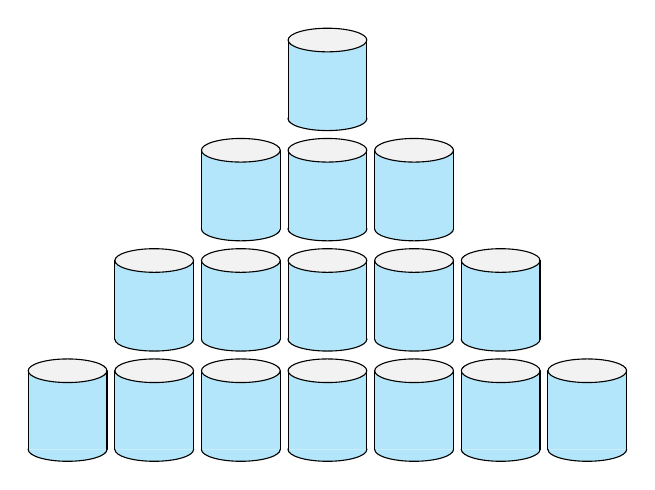
\begin{tikzpicture}[>=stealth,line join=round,line cap=round,font=\footnotesize,scale=1]
			\foreach \x/\y in {0/0,1.1/0,2.2/0,3.3/0,4.4/0,5.5/0,6.6/0}{
				\begin{scope}[shift = ({\x,\y})]
					\def\a{0.5} % ban truc lon = ban kinh tru
					\def\b{0.15} % ban truc nho
					\def\h{1} % chieu cao tru
					\path 
					(\a,\h) coordinate (D) %M -> D
					(\a,0) coordinate (C) %N -> C
					(0,\h) coordinate (O')
					(0,0) coordinate (O)
					(-\a,\h) coordinate (A) %E -> A 
					(-\a,0) coordinate (B) %F -> B
					;
					% ve day duoi
					\filldraw[fill= cyan!10,dashed] (\a,0) arc [x radius=\a, y radius=\b, start angle=0, end angle=180];
					\filldraw[fill= cyan!30] (-\a,0) arc [x radius=\a, y radius=\b, start angle=180, end angle=360];
					\fill[color = cyan!30] (A)--(B)--(C)--(D)--cycle;
					% ve day tren
					\filldraw[fill= gray!10] (0,\h) ellipse (\a cm and \b cm);
					%\draw[dashed] (O')--(O)--(C) (O)--(B);
					% ve cac canh ben
					\draw (\a,0)--(\a,\h) (-\a,0)--(-\a,\h) (A)--(B) (D)--(C);
				\end{scope}
			}
			\foreach \x/\y in {1.1/1.4,2.2/1.4,3.3/1.4,4.4/1.4,5.5/1.4}{
				\begin{scope}[shift = ({\x,\y})]
					\def\a{0.5} % ban truc lon = ban kinh tru
					\def\b{0.15} % ban truc nho
					\def\h{1} % chieu cao tru
					\path 
					(\a,\h) coordinate (D) %M -> D
					(\a,0) coordinate (C) %N -> C
					(0,\h) coordinate (O')
					(0,0) coordinate (O)
					(-\a,\h) coordinate (A) %E -> A 
					(-\a,0) coordinate (B) %F -> B
					;
					% ve day duoi
					\filldraw[fill= cyan!10,dashed] (\a,0) arc [x radius=\a, y radius=\b, start angle=0, end angle=180];
					\filldraw[fill= cyan!30] (-\a,0) arc [x radius=\a, y radius=\b, start angle=180, end angle=360];
					\fill[color = cyan!30] (A)--(B)--(C)--(D)--cycle;
					% ve day tren
					\filldraw[fill= gray!10] (0,\h) ellipse (\a cm and \b cm);
					%\draw[dashed] (O')--(O)--(C) (O)--(B);
					% ve cac canh ben
					\draw (\a,0)--(\a,\h) (-\a,0)--(-\a,\h) (A)--(B) (D)--(C);
				\end{scope}}
				\foreach \x/\y in {2.2/2.8,3.3/2.8,4.4/2.8}{
					\begin{scope}[shift = ({\x,\y})]
						\def\a{0.5} % ban truc lon = ban kinh tru
						\def\b{0.15} % ban truc nho
						\def\h{1} % chieu cao tru
						\path 
						(\a,\h) coordinate (D) %M -> D
						(\a,0) coordinate (C) %N -> C
						(0,\h) coordinate (O')
						(0,0) coordinate (O)
						(-\a,\h) coordinate (A) %E -> A 
						(-\a,0) coordinate (B) %F -> B
						;
						% ve day duoi
						\filldraw[fill= cyan!10,dashed] (\a,0) arc [x radius=\a, y radius=\b, start angle=0, end angle=180];
						\filldraw[fill= cyan!30] (-\a,0) arc [x radius=\a, y radius=\b, start angle=180, end angle=360];
						\fill[color = cyan!30] (A)--(B)--(C)--(D)--cycle;
						% ve day tren
						\filldraw[fill= gray!10] (0,\h) ellipse (\a cm and \b cm);
						%\draw[dashed] (O')--(O)--(C) (O)--(B);
						% ve cac canh ben
						\draw (\a,0)--(\a,\h) (-\a,0)--(-\a,\h) (A)--(B) (D)--(C);
					\end{scope}}
				\begin{scope}[shift = ({3.3,4.2})]
					\def\a{0.5} % ban truc lon = ban kinh tru
					\def\b{0.15} % ban truc nho
					\def\h{1} % chieu cao tru
					\path 
					(\a,\h) coordinate (D) %M -> D
					(\a,0) coordinate (C) %N -> C
					(0,\h) coordinate (O')
					(0,0) coordinate (O)
					(-\a,\h) coordinate (A) %E -> A 
					(-\a,0) coordinate (B) %F -> B
					;
					% ve day duoi
					\filldraw[fill= cyan!10,dashed] (\a,0) arc [x radius=\a, y radius=\b, start angle=0, end angle=180];
					\filldraw[fill= cyan!30] (-\a,0) arc [x radius=\a, y radius=\b, start angle=180, end angle=360];
					\fill[color = cyan!30] (A)--(B)--(C)--(D)--cycle;
					% ve day tren
					\filldraw[fill= gray!10] (0,\h) ellipse (\a cm and \b cm);
					%\draw[dashed] (O')--(O)--(C) (O)--(B);
					% ve cac canh ben
					\draw (\a,0)--(\a,\h) (-\a,0)--(-\a,\h) (A)--(B) (D)--(C);
				\end{scope}
		\end{tikzpicture}
	\end{center}
	\shortans{$68$}
	\loigiai{
		Xét cấp số cộng với số hạng đầu $u_1 = 1$, công sai $d = 2$.\\
		Khi đó, tổng của $n$ số hạng đầu cấp số cộng là $$ S_n = \dfrac{n}{2}\left[2u_1 + (n-1) d\right] \Leftrightarrow 909 = \dfrac{n}{2}[2\cdot 1 + (n - 1)\cdot 2] \Leftrightarrow 909 = n^2 \Rightarrow n = \sqrt{909} \approx 30{,}15.$$
		Suy ra $n = 30$.\\
		Do đó, số hộp sữa của dãy cuối cùng là $u_{30} = u_1 + 29d = 1 + 29\cdot 2 = 59$ hay $a = 59$.\\
		Số hộp sữa sử dụng là $S_{30} = \dfrac{30(u_1 + u_{30})}{2} = \dfrac{30(1 + 59)}{2} = 900$.\\
		Số hộp sữa thừa ra là $909 - 900 = 9$ hộp nên $b = 9$.\\
		Vậy $T = a + b = 59 + 9 = 68$.
	}
\end{ex}

%======== Câu 5
\begin{ex}%[1D2V3-8]%[KNTT - Lớp 11 - Ôn tập giữa học kì 1 - Đề 5]%[Quan Ón]
	Một người vào trường đua ngựa đặt cược, anh ta nghĩ ra một chiến lược, đó là lần đầu anh ta đặt cược $3$\$, nếu thua cược anh ta sẽ gấp $2$ số tiền cược so với lần trước đó đến khi nào thắng cược thì thôi. Anh ta đã thua $13$ lần liên tiếp và thắng cược ở lần thứ $14$. Sau đó anh ta rời khỏi trường đua. Biết rằng nếu thắng anh ta sẽ nhận được số tiền bằng đúng số tiền cược bỏ ra. Khi ra về anh ta lãi bao nhiêu tiền?
	\shortans{$3$}
	\loigiai{
		Số tiền cược của các lần liên tiếp là một cấp số nhân với $u_1 = 3$ và $q = 2$.\\
		Anh ta thua $13$ lần liên tiếp, tổng số tiền thua là 
		$$ S_{13} = u_1 + u_2 + \cdots + u_{13} = \dfrac{u_1\left(1 - q^{13}\right)}{1 - q} = \dfrac{3\left(1 - 2^{13}\right)}{1 - 2} = 24573. $$
		Số tiền anh ta cược ở lần thứ $14$ là $u_{14} = 3\cdot 2^{13}  =24576\$$.\\
		Số tiền anh ta nhận được là $u_{14} - S_{13} = 24576 - 24573  =3\$ $.\\
		Vậy anh ta đã lãi $3$\$.
	}
\end{ex}

%======== Câu 6
\begin{ex}%[1H4V2-5]%[KNTT - Lớp 11 - Ôn tập giữa học kì 1 - Đề 5]%[Quan Ón]
	Cho hình chóp $S.ABCD$, đáy là hình bình hành tâm $O$, $M$ là một điểm di động trên $SC$, $(\alpha)$ là mặt phẳng qua $AM$ và song song với $BD$. $H$ và $K$ lần lượt là giao điểm của $(\alpha)$ với $SB$, $SD$. Tính giá trị của $T = \dfrac{SB}{SH} + \dfrac{SD}{SK} - \dfrac{SC}{SM}$.
	\shortans{$1$}
	\loigiai{
	\immini{
		Giả sử $AM$ cắt $SO$ tại $I$.\\
		$(\alpha)$ qua $AM$ và song song với $BD$, nên $(\alpha)$ cắt mặt phẳng $(SBD)$ theo giao tuyến $HK$ qua $I$ và \\$HK\parallel BD$ ($H$ trên $SB$ và $K$ trên $SD$).\\
		Ta có $\dfrac{SB}{SH} = \dfrac{SD}{SK} = \dfrac{SO}{SI} \Rightarrow \dfrac{SB}{SH} + \dfrac{SD}{SK} = \dfrac{2SO}{SI}$.\\
		Dựng $OL \parallel AM$, ta có $L$ là trung điểm $CM$\\
		$\Rightarrow LM = LC$.\\
		Ta có $\begin{aligned}[t]
			\dfrac{SO}{SI} = \dfrac{SL}{SM} = \dfrac{SC-LC}{SM} &=& \dfrac{SC}{SM} - \dfrac{LC}{SM} \\
			&=& \dfrac{SC}{SM} - \dfrac{ML}{SM}.
		\end{aligned}$
	}{
		\begin{tikzpicture}[>=stealth,line join=round,line cap=round,font=\footnotesize,scale=1]
			\path 
			(0,0) coordinate (D)
			(-1.6,-1.5) coordinate (A)
			(1.9,-1.5) coordinate (B)
			($(D)-(A)+(B)$) coordinate (C)
			(intersection of A--C and B--D) coordinate (O)
			($(O)+(-0.4,3.4)$) coordinate (S)
			($(S)!0.45!(D)$) coordinate (K)
			($(S)!0.45!(B)$) coordinate (H)
			(intersection of K--H and S--O) coordinate (I)
			(intersection of A--I and S--C) coordinate (M)
			($(M)!0.5!(C)$) coordinate (L)
			;
			\draw (S)--(A)--(B)--(C)--(S)--(B) (A)--(H)--(M);
			\draw[dashed] (C)--(A)--(D)--(C) (B)--(D)--(S)--(O)--(L) (K)--(A)--(M)--(K)--(H);
			\foreach \x/\g in {A/-135,B/-45,C/0,D/40,M/45,O/-100,S/90,I/180,H/-30,L/45}\fill[black] (\x) circle (1pt)+(\g:3mm) node[scale=0.8]{$ \x $};
			\fill[black] (K) circle (1pt)+(180:2mm) node[scale=0.8]{$K$};
		\end{tikzpicture}
	}
	\noindent
	Mà $\dfrac{ML}{MS} = \dfrac{OI}{SI} \Rightarrow \dfrac{SO}{SI} = \dfrac{SL}{SM} = \dfrac{SC}{SM} - \dfrac{IO}{SI} = \dfrac{SC}{SM} - \dfrac{SO-SI}{SI}$\\
	$\Rightarrow \dfrac{SO}{SI} = \dfrac{SC}{SM} - \dfrac{SO}{SI} + 1 \Rightarrow \dfrac{2SO}{SI} - \dfrac{SC}{SM} = 1$\\
	Vậy ta có $\dfrac{SB}{SH} + \dfrac{SD}{SK} - \dfrac{SC}{SM} = 2\dfrac{SO}{SI} - \dfrac{SC}{SM} = 1$.
}
\end{ex} 

\Closesolutionfile{ans}

\indapan{6}{ans-KQ}